\section{Scientific Background} \label{sec:theory}
% Physics part
% - Composition (photometry) -> telescope optics?/instrument?/bit depth?
% - Trajectories and relative trajectory of spacecraft, especially trajectories for flybys
% - Star rendering?
% - Describe physics of SSSBs, i.e. size/shapes/surface (features/color/albedo) illumination
%
% Computer Science part
% - Physics-based rendering? -Shaders/procedural terrain generation
% - Compression
% - Reconstruction (SfM), relates to camera physics. Generally Computer Vision topic.
% - Image processing Gaussian filtering, downscale local means
% - Logic for choosing number of reconstructed points as quality measure
%
% Space
% - Small Spacecrafts -> small data budgets?
%
% Max Science?
%
% Concepts to describe???

\subsection{Small Solar System Bodies}
The \gls{iau} defines an \gls{sssb} as any object in the Solar System, that is not a planet, dwarf planet or satellite~\cite{iau_sssb}. Within this work, the term \gls{sssb} mostly refers to asteroids and comets.

In a classical definition, asteroids and comets were two distinct \gls{sssb} classes based on observational, physical and dynamical properties. However, the discovery of active asteroids and dormant comets began to blur these definitions. Many observed objects cannot be strictly classified into the classical categories anymore. Therefore these objects are more frequently described as part of an asteroid-comet continuum with asteroids and comets at the ends of the continuum~\cite{Hsieh2017Asteroid-cometSystem}.

Despite the shift towards a continuum definition, the classical definition is used in this work. Non-active objects are referred to as asteroids and active objects are referred to as comets where it is necessary to distinguish these types of objects. Consequently, a description following the classical definition of asteroids and comets is provided.

\subsubsection{Asteroids}
Asteroids are rocky bodies that mostly reside in an orbit between Mars and Jupiter, i.e. the asteroid main belt. More than \SI{930000}{} asteroids are known of which more than \SI{540000}{} are numbered. The ephemeris of more than \SI{930000}{} and absolute magnitude of more than \SI{925000}{} is known. However, physical parameters like diameter ($> \SI{136000}{}$), albedo ($> \SI{135000}{}$), rotation period ($> \SI{19000}{}$), spectral type ($> \SI{2000}{}$) and the standard gravitational parameter ($> \SI{10}{}$) are known for only a small fraction of asteroids~\cite{JPLEngine}.

Asteroids are often referred to as rubble piles, i.e. objects which gravitationally aggregated boulders resulting in a low bulk density because of many void spaces in their internal structure~\cite{Richardson2002GravitationalEvolution}. An example of rubble pile asteroids are Bennu and Ryugu due to their low density~\cite{Chesley2014OrbitBennu, Watanabe2019Hayabusa2Pile}.

\subsubsection{Comets}
Comets are small icy bodies that mostly reside farther away from the Sun than asteroids. Inside the heliosphere, the source of comets is the Kuiper belt while comets from outside the heliosphere are thought to originate in the \"Opik-Oort cloud. Comets are occasionally perturbed by the gravity of other objects which moves their orbits closer to the Sun. While being close to the Sun, volatiles begin to evaporate which creates the well-known coma around the nucleus. In most cases the coma is several orders of magnitudes larger than the nucleus. The size of nuclei is on the order of a few kilometres while comas can extend hundreds of thousands of kilometres. Additionally, a gas and a dust tail are formed. The gas tail originates from coma charged particles that are carried away from the nucleus by the magnetic field carried by the solar wind. The dust tail is formed by small dust particles in the coma which are carried away from the nucleus by the solar radiation pressure. Larger dust particles remain along a comets trajectory as a trail forming part of the meteoroid environment. If a comet is heated unevenly, trapped gas escapes at weak spots in the surface forming jets of gas and dust~\cite{Comets, a2017comets, Soja2019IMEM2:System}.

Physical parameters of comets are not well-known, since comet nuclei are small. It is difficult to image a comet nucleus when it moves closer to the Sun since the nucleus is surrounded by the coma. Approximately \SI{3500}{} comets are known of which more than \SI{400}{} are numbered~\cite{JPLEngine}. The ephemeris ($> \SI{1700}{}$) and magnitude ($>\SI{1300}{}$) are known for many comets. Only a few comets have known physical properties like the diameter ($> \SI{100}{}$) or the rotation period ($> \SI{20}{}$)~\cite{JPLEngine}.

It is not clear whether comets are generally similar to rubble piles or rather consolidated, monolithic bodies. It is assumed that most bodies in the range of \SI{200}{\meter} to \SI{10}{\kilo\meter} are rubble piles~\cite{Walsh2018RubbleAsteroids}. However, density measurements and surface features of \gls{67p} are not conclusive so far~\cite{Weissman2020OriginNuclei}. 

\subsubsection{Orbital Mechanics} \label{sec:orbit_mechanics}
All objects in space move on trajectories, following the Kepler equations. Trajectories are commonly defined using six orbital elements. Semi-major axis \gls{a}, eccentricity \gls{e}, inclination \gls{i}, right ascension of ascending node \gls{Omega}, argument of periapsis \gls{omega} and the true anomaly \gls{nu} or mean anomaly \gls{M} at a given epoch. This parameterisation is also called modified Keplerian elements~\cite{Hintz2015FundamentalsAstrodynamics}. Figure~\ref{fig:kepler_elements} shows the geometric relations of the angular elements.
\begin{figure}[htb]
    \centering
    \begin{subfigure}[b]{0.47\textwidth}
        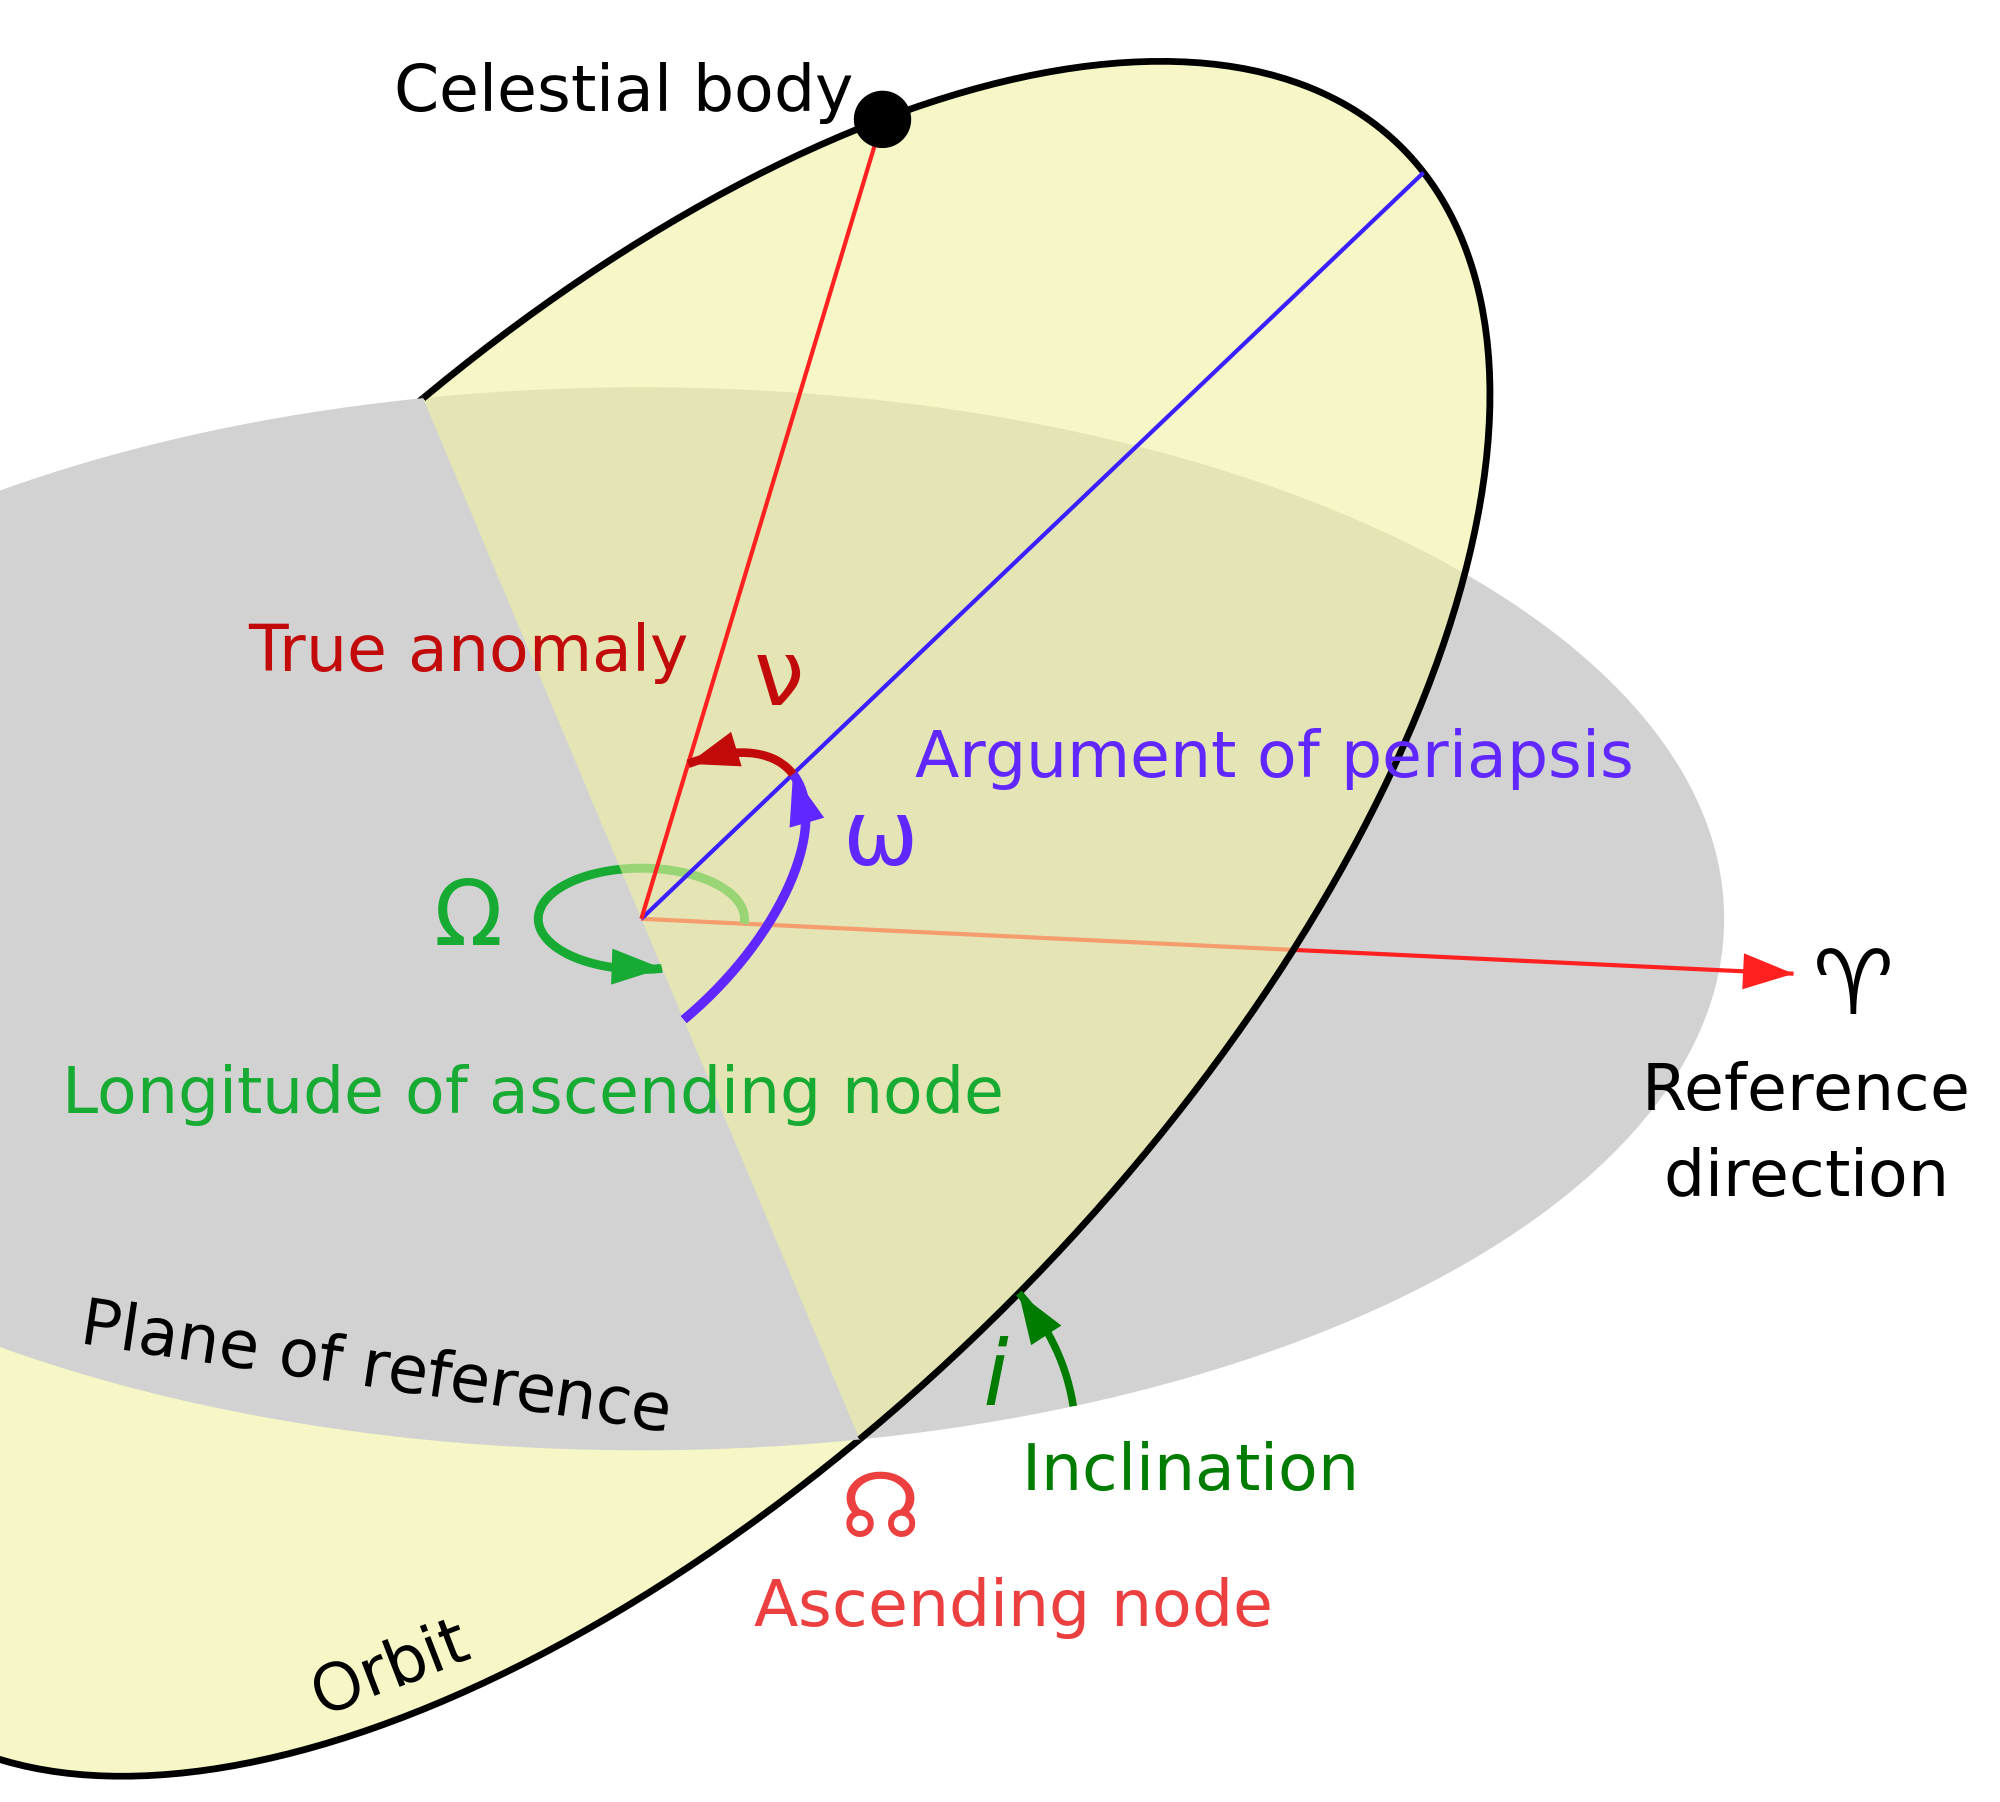
\includegraphics[width=.8\textwidth]{doc/thesis/0_figures/Orbit_elements.png}
        \caption{}
        \label{fig:kepler_elements}
    \end{subfigure}
    \begin{subfigure}[b]{0.47\textwidth}
        \centering
        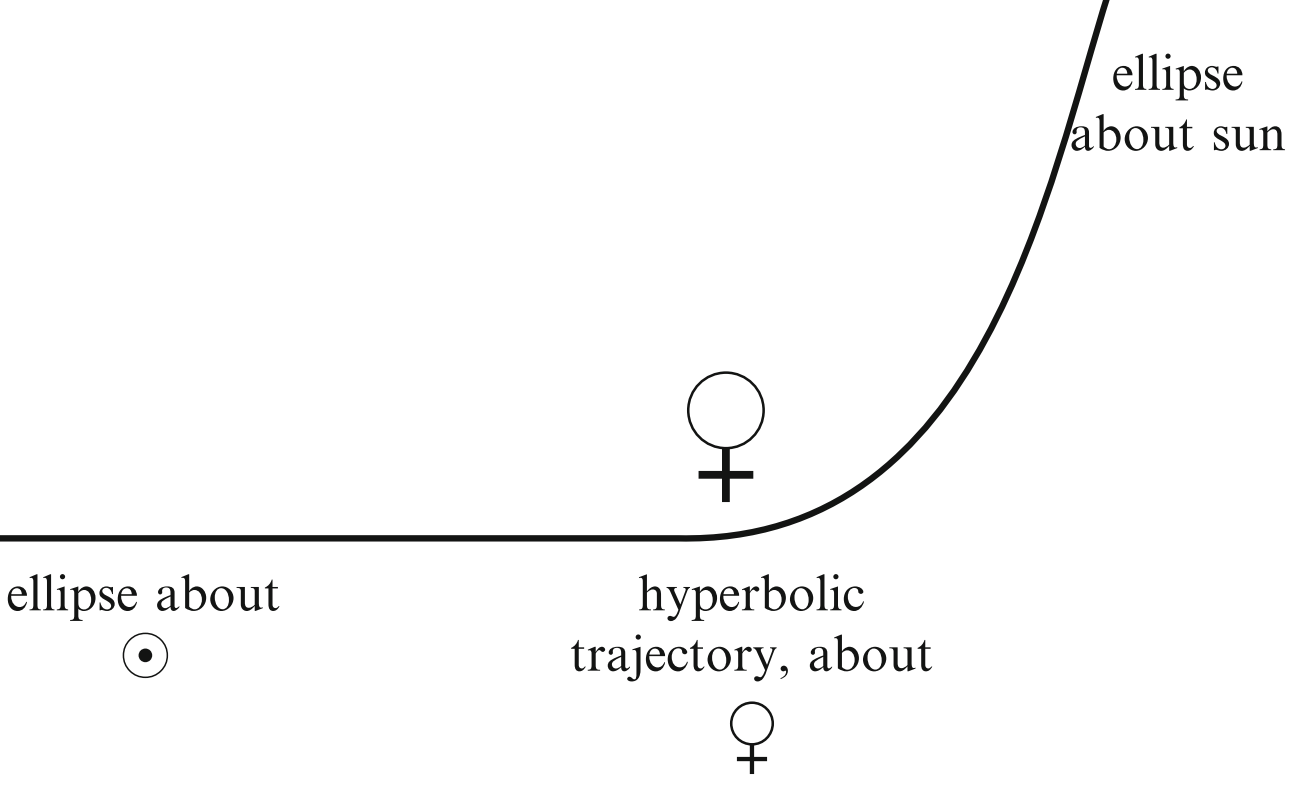
\includegraphics[width=\textwidth]{doc/thesis/0_figures/Hyperbolic_trajectory.png}
        \caption{}
        \label{fig:hyperbolic_orbit}
    \end{subfigure}
    \label{fig:astrodynamics}
    \caption{Important astrodynamic definitions and relations. (a) Modified Keplerian elements \cite{Commons2019Orbit}. (b) A closed orbit around the Sun (\gls{sun}) becomes a hyperbolic trajectory around another body, in this example Venus (\gls{venus})~\cite{Hintz2015FundamentalsAstrodynamics}.}
\end{figure}

Fly-by scenarios in the Solar System are often closed orbits around the Sun, i.e. \gls{e}$_{\astrosun} < 1$ while they are hyperbolic trajectories in the reference frame of the target, i.e. \gls{e}$_{\venus} > 1$. An example is given in Figure~\ref{fig:hyperbolic_orbit}. A high relative velocity and the small gravitational force exerted by a \gls{sssb} result in a trajectory closer to a straight line than the bend trajectory presented in Figure~\ref{fig:hyperbolic_orbit}. 

Most asteroids move on orbits with low eccentricity while most comet orbits have high eccentricities~\cite{ChamberlinCometDistribution}. The eccentricity distribution is caused by the origin of asteroids and comets. While asteroids mostly originate from the main belt which is a nearly circular region, comets enter the inner Solar System from far out, i.e. comets' aphelion is far from the Sun resulting in high eccentricities.

\subsection{Image Rendering}
Rendering is the process of creating \gls{2d} images from \gls{3d} objects. A virtual \gls{3d} world with objects is created which is used to calculate \gls{2d} images. Light sources and cameras produce artificial illumination and define which part of the world is being captured. A rendering engine calculates the pixel values to generate the final image based on energy conservation by using the rendering equation~\cite{Kajiya1986TheEquation}.

\subsubsection{Path Tracing}
Path tracing is a special form of ray tracing. Ray tracing is a rendering technique where the path of light rays is traced to generate pixels while simulating effects of encounters with objects. Path tracing does not branch into an exponentially growing number of rays when being reflected or refracted but only a single path is followed. Path tracing cuts computation time dramatically compared to ray tracing in scenes with a lot of reflection, refraction and shadow rays per pixel~\cite{Kajiya1986TheEquation}. Path tracing can simulate different effects, such as reflection, refraction, scattering and dispersion. There are four types of rays: camera rays, reflection rays, transmission rays and shadow rays. Reflection and transmission can be further categorised as either diffuse, glossy or singular. Path tracing is a popular rendering technique where a high degree of realism is necessary since it is a realistic simulation of light transport. However, the high degree of realism created by path tracing requires substantial computational power~\cite{Vasiou2018ACost}.

\subsubsection{3D Models and Shaders}
A \gls{3d} model is a set of vertices in \gls{3d} space linked by surfaces. The most common type of \gls{3d} models are polygonal meshes. Polygonal meshes are shell models that consist of polygons. A vertex is a corner of a polygon, i.e. every triangle has three vertices and every tetrahedron has four vertices. A face refers to the surfaces that make up a \gls{3d} model. Depending on the rendering environment, \gls{3d} models can have varying levels of detail and their surface can have different properties such as reflection, refraction and transmission~\cite{FoundationCyclesIntroduction}.

A shader is used to calculate effects of interactions of rays and objects during the rendering process. Shaders provide a flexible method to influence the rendering outcome during the rendering process. Shaders can be used to change the positions of vertices, colours, lighting and surface properties by using equations. Complex surface structures and texture can be generated procedurally with shaders. Shaders are commonly executed on \glspl{gpu} since \gls{gpu} hardware is well suited for this task~\cite{Pharr2010ChapterMaterials, Sans2017ACUDA, Spath2018AdvancedThMAD}.

Shaders that influence the surface of an object use a \gls{bsdf}. \glspl{bsdf} are a mathematical functions that describe light scattering behaviour of surfaces of \gls{3d} models. Several shader classes such as diffuse, glossy, refraction and transparent shaders create the respective effect based on \glspl{bsdf}~\cite{FoundationCyclesIntroduction, Pharr2010ChapterMaterials}.

\subsubsection{Field of View}
The \gls{fov} defines the visible extent of a camera view in \gls{3d} scene. Vectors that point to the edges of the \gls{fov} can be constructed from geometric considerations resulting in
\begin{align}
    e_{i} = v_d \pm \frac{v_j \times s_k}{2 \times f}, \label{eq:fov_edge}
\end{align}
where $e_{i}$ is a vector for the $i^{th}$ edge of the \gls{fov}, $v_d$ is the direction vector of the camera, $v_j$ is the vector pointing right or up in the \gls{fov} plane, $s_k$ is the camera sensor width or height and $f$ is the focal length. The left and right edge vectors, $e_{left}$ and $e_{right}$, are calculated with the vector $v_r$ pointing right in the \gls{fov} plane and the sensor width $s_w$. The upper and lower edge vectors, $e_{upper}$ and $e_{lower}$  are calculated with the vector $v_r$ pointing up in the \gls{fov} plane and the sensor height $s_h$.

In addition to the extent of the \gls{fov} within the image plane, rendering requires the \gls{fov} to be clipped to a minimum and maximum distance. Clipping defines which objects appear in a rendered scene. Clipping is necessary to limit the required computational power for rendering. 

\subsubsection{Photometric calibration} \label{sec:photo_cal}
Photometric calibration is the process of correcting raw images from a sensor to a common level of brightness. Differences can originate from varying exposure times, gains or different camera sensors~\cite{Bergmann2018OnlineSLAM}. Photometric calibration uses a photometric system, such as the \gls{ubv}, which are reference systems with which star magnitude measurements can be compared for a given band of the system~\cite{Bessell1979UBVRIPhotometry}.

The apparent magnitude of a star is converted into photon flux density \gls{flux_d} relative to magnitude 0 by using,
\begin{align}
    F = 10^{-0.4 \times m}, \label{eq:mag_flux}
\end{align}
where \gls{m} is the apparent star magnitude. Given the apparent magnitude of a specific band, the photon flux density \gls{flux_d} of a reference object can be calculated using
\begin{align}
    F = F_0 \times \frac{\Delta\lambda}{\lambda} \times 10^{-0.4 \times m}, \label{eq:comp_flux_0mag}
\end{align}
where \gls{flux_0} is the photon flux density at magnitude 0, \gls{dlambda} is the wavelength bandwidth, \gls{lambda} is the centre wavelength and \gls{m} is the object's magnitude. The required constants to calculate the photon flux of an object from its magnitude in a given band are presented in Table~\ref{tab:ubv_constants}.

\begin{table}[htb]
    \centering
    \caption{Constants for calculating photon fluxes using the \gls{ubv}~\cite{Bessell1979UBVRIPhotometry}.}
    \label{tab:ubv_constants}
    \begin{tabular}{l|l|l|l}
        \textbf{Band} & \textbf{Centre wavelength \gls{lambda} [\SI{}{\nano\meter}]} & \textbf{$F_0$ [\SI{1e-26}{\watt\per\square\meter\per\hertz}]} & \textbf{$\frac{\Delta\lambda}{\lambda}$}[~] \\ \hline
        U             & 0.36                       & 1810        & 0.15             \\
        B             & 0.44                       & 4260        & 0.22             \\
        V             & 0.55                       & 3640        & 0.16            
    \end{tabular}
\end{table}

Consequently, the reference photon flux for one pixel of the \gls{ccd} \gls{fref} is calculated using
\begin{align}
    F_{ref} = F \times \frac{A \times A_{pixel}}{f^2 \times \pi}, \label{eq:comp_flux_pix}
\end{align}
where \gls{flux_d} is the photon flux density, \gls{a} is the aperture area, \gls{a_pixel} is the area of a pixel and \gls{f} is the focal length of the instrument.

In the last step, the calibration factor~\gls{calibfactor} is calculated. It is defined as
\begin{align}
    f_c = \frac{F_{ref} \times \alpha}{I_{ref}}, \label{eq:comp_cal_fac}
\end{align}
where \gls{fref} is the reference flux, \gls{alpha} is the albedo and \gls{iref} is the reference intensity. Multiplying the image with \gls{calibfactor} produces the calibrated image.

The effect of photometric calibration is delineated in Figure~\ref{fig:t_photometry}. Photometric calibration corrects the brightness difference of a set of images towards a common brightness level~\cite{Bergmann2018OnlineSLAM}.
\begin{figure}[htb]
    \centering
    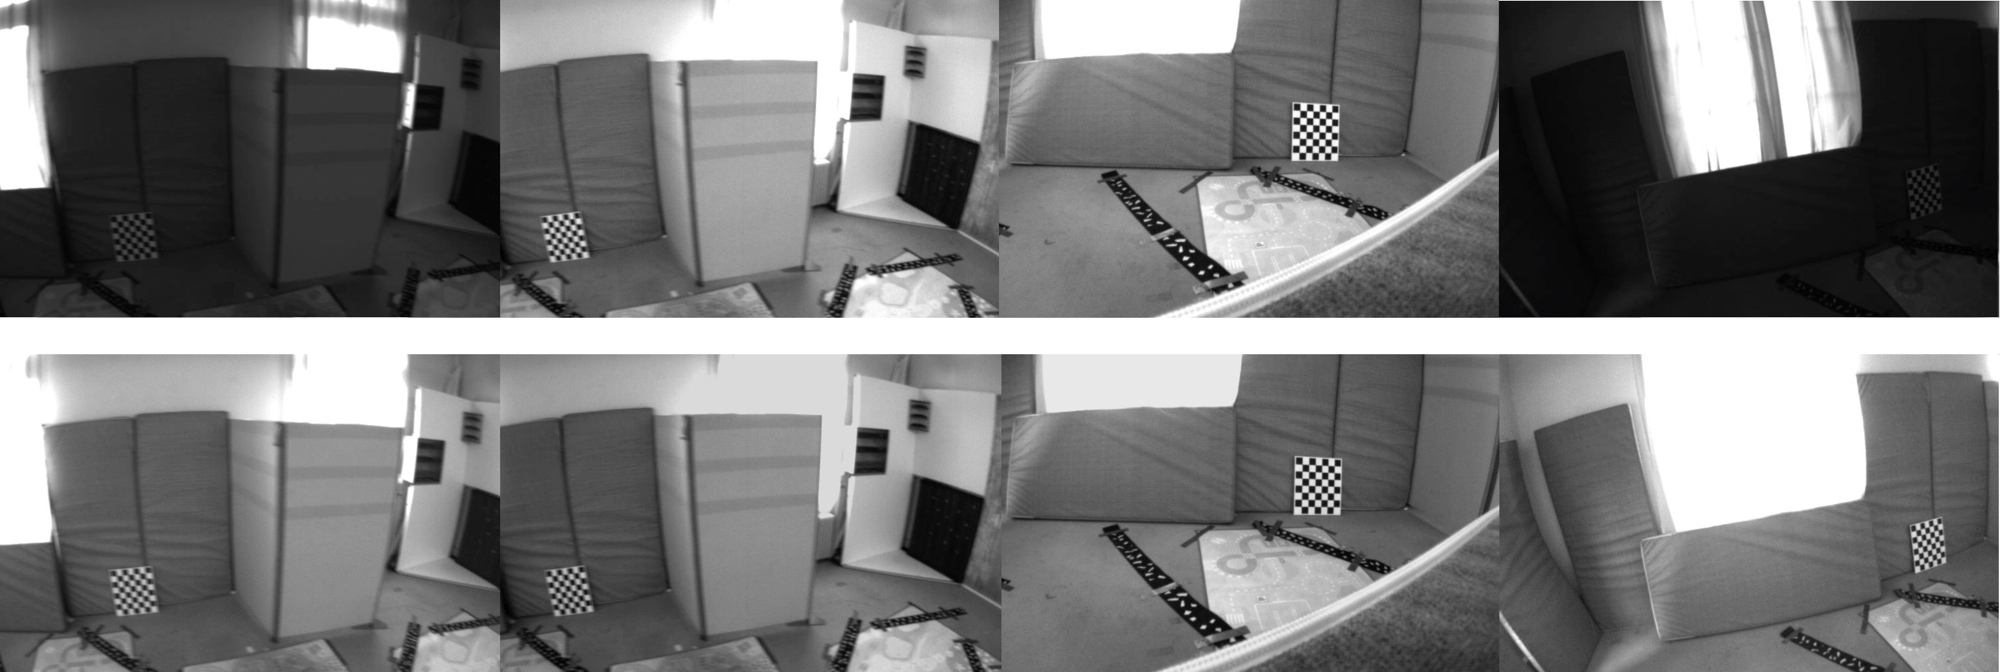
\includegraphics[width=\textwidth]{doc/thesis/0_figures/photo_calib.jpg}
    \caption{Image series before (top) and after (bottom) photometric calibration which eliminated the brightness differences~\cite{Bergmann2018OnlineSLAM}.}
    \label{fig:t_photometry}
\end{figure}

\subsection{Computer Vision} \label{sec:t_cv}
\Gls{cv} is the science of extracting information from digital photos and videos by mimicking the human vision system using a computer. \Gls{cv} encompasses a wide field of activities, from image formation, processing, detecting and matching features, image segmentation and \gls{3d} reconstruction~\cite{szeliski2010computer}. \Gls{cv} is computer based photogrammetry which aims to obtain information about physical objects and the environment from photographic images~\cite{Kasser2002DigitalPhotogrammetry}. A common approach for \gls{3d} reconstruction is stereo-photogrammetry, also referred to as computer stereo vision. Stereo-photogrammetry applies the binocular vision principle of the human vision system to obtain structural information from images~\cite{do2019review}. Since most, if not all, deep space missions have a visual imager instrument on-board, \gls{cv} provides a useful framework to obtain the \gls{3d} structure of an observation target. A similar approach is \gls{sfm} where the camera motion creates the stereo perspective.

\subsubsection{Pinhole Camera Model}
All \gls{cv} problems require a camera model. The most commonly used model in \gls{cv} is the pinhole camera. Figure~\ref{fig:pinhole_cam} presents an overview of the important elements of the pinhole model \cite{sturmCameraModel}.

\begin{figure}[htb]
    \centering
    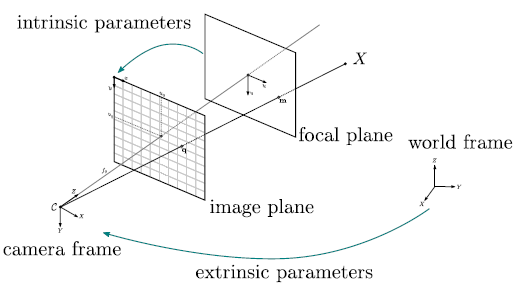
\includegraphics[width=.85\textwidth]{doc/thesis/0_figures/sfm/pinholeCamera.png}
    \caption{Overview of the components of the pinhole camera model. Intrinsic camera parameters model optical distortions, extrinsic parameters model camera position and orientation. The image plane is where the light sensor is. Locations in the image plane are described with u,v-coordinates. The focal plane is where the focus of the optical system is. The thin line from the origin of the camera frame through the centres of the image and focal plane is the optical axis~\cite{OpenMVGCameras}.}
    \label{fig:pinhole_cam}
\end{figure} 

The pinhole camera model can be described using the $3\times4$ camera matrix \gls{k} defined as
\begin{align}
    \textbf{K} = \begin{bmatrix}
        f\times k_u & 0           & c_u \\
        0           & f\times k_v & c_v \\
        0           & 0           & 1   \\
    \end{bmatrix} 
    \begin{bmatrix}
        \textbf{R} & t
    \end{bmatrix}, \label{eq:camera_m}
\end{align}
where \gls{f} is the distance between the focal plane and the image plane, \gls{k_u} and \gls{k_v} are scaling factors, \gls{c_u} and \gls{c_v} are the coordinates of the principle point on the image plane, \gls{r} is a $3\times3$ rotation matrix and \gls{t} being a $3\times1$ translation vector. The first matrix of \gls{k} reflects the camera intrinsic parameters while the second matrix describes the extrinsic parameters.
More sophisticated pinhole camera models include distortions. Distortions can include one or more factors for radial and tangential distortions. A special case with three radial and two tangential distortion factors is called Brown T2 model~\cite{OpenMVGCameras, sturmCameraModel}.

The conversion between object coordinates and image coordinates is obtained from geometric considerations of the pinhole camera model shown in Figure~\ref{fig:pinhole_cam} and is defined as
\begin{align}
    u_{pix} = \frac{f}{s_w} \times \frac{\hat{v}_r \cdot p}{\hat{v}_d \cdot p + 1} \times (r_u - 1), \label{eq:pix_conversion} 
\end{align}
%x_pix = ss * (f_over_w_ccd_2 * np.dot(right_norm, vec) / np.dot(direction, vec) + 1.) * (res_x - 1) / 2.
where \gls{u_pix} is the u-coordinate of a pixel in the image frame, \gls{f} is the focal length, \gls{s_w} is the sensor width, \gls{v_rhat} is the unit vector pointing right in the image plane, \gls{p} is the Cartesian coordinate vector of a star, \gls{v_d} is the vector of the optical axis and \gls{r_u} is the number of pixels in u-direction. Similarly, the conversion for v-coordinate of a pixel \gls{v_pix} is obtained by replacing the sensor width \gls{s_w} with the sensor height \gls{s_h}, \gls{v_rhat} by the unit vector \gls{v_uhat} pointing up in the image plane and the number of pixels in u-direction \gls{r_u} by the number of pixels in the v-direction \gls{r_v}. The vectors \gls{v_rhat} and \gls{v_uhat} are calculated by subtracting \gls{v_d} from the field of view edge vectors \gls{e_right} and \gls{e_upper} as defined in Equation~\ref{eq:fov_edge}.

\subsubsection{Structure-from-Motion}
\Gls{sfm} can be considered the inverse process to rendering, i.e. creating \gls{3d} models from \gls{2d} images. \Gls{sfm} uses multiple views of the same object from different camera positions to reconstruct an object's geometry. \Gls{sfm} recovers the \gls{3d} structure of an object and the camera poses of each image~\cite{szeliski2010computer}. Depth information is obtained through the motion parallax created by the moving camera. Generic steps of an \gls{sfm} processing pipeline are presented in Figure~\ref{fig:sfm_steps}.

\begin{figure}[htb]
    \centering
    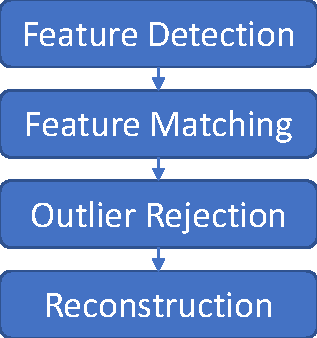
\includegraphics[width=.25\textwidth]{doc/thesis/0_figures/sfm/SfM.pdf}
    \caption{Generic steps of a \gls{sfm} processing pipeline.}
    \label{fig:sfm_steps}
\end{figure}

Figure~\ref{fig:sfm_geometry} shows a generic observation geometry in an \gls{sfm} problem. Various images containing feature points of the same object point are taken from varying positions. Lines connecting the features points and object point depict the relation between \gls{2d} feature points and a \gls{3d} object point. 

\begin{figure}[htb]
    \centering
    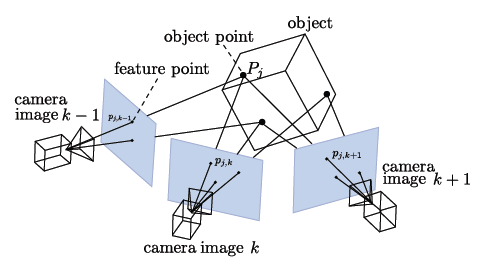
\includegraphics[width=\textwidth]{doc/thesis/0_figures/sfm/sfm_geometry.png}
    \caption{Generic observation geometry in a \gls{sfm} problem. The \gls{3d} structure can be reconstructed from several point observations and intrinsic camera parameters~\cite{OpenMVGSfm}.}
    \label{fig:sfm_geometry}
\end{figure}

Reconstructing \gls{3d} points from an image series requires finding correspondence between images. Correspondence is found by detecting and matching features in multiple images. A feature point is a local, meaningful and detectable part of an image. Feature points are also referred to as key-points or interest-points. Features can be image regions of sudden change, shape features or texture contours. Commonly detected features are corners, edges, junctions, blobs and lines~\cite{Tareen2018ABRISK}. Feature descriptors assign a distinct identity features after feature description for later matching. A range of feature description algorithms exist. Most feature descriptors are combined with a distinct feature detector. However, detectors and descriptors can be interchanged. Feature detectors are tasked with detecting feature-points in an image. A common requirement for feature descriptors and detectors is scaling, rotation and affine invariance. The most prevalent feature detector-descriptor pairs are \gls{sift}, \gls{surf}, \gls{orb}, KAZE and \gls{akaze}~\cite{Tareen2018ABRISK}.
% Add SIFT description?
After detection and description of all images, features are matched, i.e. an algorithm identifies the same feature in multiple images. Either an L1 or L2-norm for scalar descriptors or the hamming distance for binary descriptors are used. Feature matching can use image pairs or a series of images. Various geometries can be described using different mappings. The homography matrix \gls{H_m} describes a coordinate mapping of two different views and is defined as
\begin{align}
    x'_i = \textbf{H}x_i, \label{eq:homography_m}
\end{align}
where \gls{x_i}$'$ are the coordinates of point $i$ in the second image, \gls{x_i} are the coordinates of point $i$ in the first image and \gls{H_m} is the homography matrix. However, \gls{H_m} describes only a purely rotating or moving camera capturing a planar scene~\cite{schonberger2016structure}. The fundamental matrix \gls{F_m} describes the relation between two images of the same scene for a moving camera. It relates points of uncalibrated images and is defined as
\begin{align}
    {x'_i}^{T}\textbf{F}x_i = 0, \label{eq:fundamental_m}
\end{align}
where \gls{x_i}$'$ are the coordinates of point $i$ in the second image, \gls{x_i} are the coordinates of point $i$ in the first image and \gls{F_m} is the fundamental matrix. The epipolar line \gls{l_i} constitutes all possible locations of point \gls{x_i}$'$. The epipolar line is defined as
\begin{align}
    l'_i = \textbf{F}x_i, \label{eq:epipolar_l}
\end{align}
where \gls{F_m} is the fundamental matrix and \gls{x_i} are the coordinates of a point in the first image.

Taking into account the camera intrinsic parameters, the fundamental matrix \gls{F_m} becomes the essential matrix \gls{E_m} which is defined as
\begin{align}
    \textbf{E} = (\textbf{K}')^{T}\textbf{F}\textbf{K}, \label{eq:essential_m}
\end{align}
with \gls{k}$'$ being the camera matrix of the second view, \gls{F_m} being the fundamental matrix as defined in Equation~\ref{eq:fundamental_m} and \gls{k} being the camera matrix of the first view. The essential matrix is intended to be used in conjunction with calibrated images where the camera intrinsic parameters are available.

If sufficient points are correctly mapped using one of the transformations from Equations \ref{eq:homography_m}, \ref{eq:fundamental_m} and \ref{eq:essential_m}, the points are geometrically verified. However, geometric verification does not necessarily remove all outliers. Therefore, outlier rejection is performed to remove incorrect matches. Several algorithms such as \gls{ransac}~\cite{Fischler1981RandomCartography}, \gls{acransac}~\cite{moisan2012automatic}, \gls{msac}~\cite{wang2009generalized} and \gls{prosac}~\cite{Chum2005MatchingConsensus} are used for outlier removal. These outlier rejection algorithms attempt to robustly estimate the correct model and remove outliers. The result of outlier rejection is the view graph which relates different views to each other with images as nodes and pairs as edges~\cite{schonberger2016structure}.

The reconstruction process produces a \gls{3d} point cloud based on the view graph. A point cloud is a set of independent points with coordinates in \gls{3d} space. Two principle methods for \gls{sfm}-based reconstruction exist, incremental and global. For unorderd image sets the incremental approach is used more frequently~\cite{schonberger2016structure}.

Incremental reconstruction starts with an initial view pair. Selecting the initial pair is a critical step because the reconstruction algorithm might not converge after using a bad initial pair. Typically, starting with a scene with many overlapping camera views constitutes a robust initialisation and results in higher accuracy because of redundant information from many images~\cite{schonberger2016structure}.
Subsequently, additional images are registered to the model based on corresponding features which can be used to triangulate additional points in already registered images. The triangulation step can include estimating camera poses and camera intrinsic parameters for uncalibrated images. Triangulation is an essential step of making \gls{sfm} robust by adding redundant information about existing points to a model and adding additional points which increases the coverage of a model~\cite{schonberger2016structure}.

Image registration and triangulation are separate processes although their results are linked. Errors of one process can increase the error of the other process. If pose estimation during image registration is erroneous, the error propagates to the location estimate of a triangulated point. Bundle adjustment is often employed to increase robustness of this step. Bundle adjustment is the combined refinement of camera pose and point position estimate. A frequently used error minimisation algorithm is the Levenberg-Marquardt algorithm ~\cite{schonberger2016structure, Moulon2013AdaptiveEstimation}.

Global \gls{sfm} pipelines try to eliminate the problem of accumulating errors of incremental \gls{sfm} by using a common reference frame for all views. While incremental reconstruction accumulates errors with every added view, global reconstruction attempts to distribute these residuals equally for all reconstructed points~\cite{Moulon2013GlobalMotion}. Global \gls{sfm} pipelines calculate the essential matrix for all image pairs in the initial step. Rotation estimation is often separated from translation and structure estimation. First a consistent set of rotations is computed in a global frame based on relative rotations of input pairs. Second, camera translations and the object structure are estimated.

Stability of either \gls{sfm} approach can be improved by providing priors for the camera intrinsic and extrinsic parameter estimation which are then used as initial guess for the optimisation process~\cite{Irschara2011EfficientPriors}.

Incremental and global \gls{sfm} methods create a sparse point cloud and estimate the intrinsic and extrinsic camera parameters. The sparse point cloud can be densified using \gls{mvs} techniques~\cite{Pagani2011DenseImages}. Image pairs with established camera positions are used to calculate depth maps. The depth maps are fused and filtered to increase the number of points in the point cloud. Point cloud densification mimics human depth perception and leverages the information to improve the accuracy of point clouds.

Subsequently, a point cloud is converted into a \gls{3d} model by estimating a mesh surface from the point cloud. Outliers are detected and removed from the scene during mesh creation. Different approaches exist which yield different results. Some techniques only use strongly supported faces, i.e. faces that are supported by many points of a point cloud. Other methods include weakly supported surfaces due to e.g. obstructions~\cite{Jancosek2014ExploitingSurfaces}. The output of mesh creation is a rough surface model of a 3D object.

A frequently used mesh creation algorithm is Delaunay tetrahedralisation. Delaunay tetrahedralisation is a triangulation method in which a set of points \gls{P} is triangulated to not contain any point of \gls{P} within the circumscribed sphere of any tetrahedron (3-simplex). Delaunay tetrahedralisation is a frequently used algorithm because it provides a unique solution to the triangulation problem~\cite{vu2012high}.

The accuracy of a rough surface model can be increased with mesh refinement. In cases where a sparse point cloud was used to create the rough mesh, refinement can improve the model accuracy substantially. One such algorithm for mesh refinement is variational multiview stereovision. Initial mesh creation captures the main features of a structure hence variational multiview stereovision can employ local optimisation algorithms since local optimisation is unlikely to be trapped in local minima~\cite{Faugeras1998VariationalProblem, vu2012high}.

The final step in \gls{3d} reconstruction is texturing the surface model. Ideally, camera poses and surface models are exact. However, frequently texturing needs to cope with inacurate camera poses and surface models. Likewise, effects such as differing illumination and exposure, unreconstructed occluding objects or varying image scales need to be addressed. Texturing is often separated in image selection and optimising the resulting image set for consistency~\cite{Waechter2014LetReconstructions}. Image selection algorithms are categorised into two types. One type blends multiple images per face to achieve consistent texture across patches. The other type uses a single image per face~\cite{Waechter2014LetReconstructions}.
Subsequently, colours differences originating from exposure and illumination variations need to be adjusted. Seams between patches are corrected by photometric adjustments. Colour adjustment can be split into local or global adjustments. Local adjustment smooths the transition between texture patches by introducing gradients in texture luminances, e.g. example with heat diffusion equations~\cite{Velho2007ProjectivePhotography}. Global adjustment methods calculate the luminance correction terms for a global optimum~\cite{Lempitsky2007SeamlessMaps}.

\subsection{Image Compression and Processing}
Digital image processing uses computers to process digital images through algorithms. Processing techniques relevant to this thesis are image compression (cf. Section~\ref{sec:t_compress}), Gaussian filtering  (cf. Section~\ref{sec:t_gauss}) and image down-sampling  (cf. Section~\ref{sec:t_downsample}).

\subsubsection{Image Compression} \label{sec:t_compress}
Data compression is tasked with encoding information using less bits than the original representation. Other terms for data compression are source coding or bit-rate reduction~\cite{Mahdi2012ImplementingTechnique}. Two principle methods of compression exist, lossless and lossy compression. While it is possible to recover all information after lossless compression, lossy compression accepts a certain irreversible loss of information to achieve higher compression ratios.

Lossless compression leverages statistical redundancy in data to decrease the number of bits necessary to encode the same information in a reversible process. Many lossless compression algorithms exist such as Huffman coding, arithmetic coding or Lempel-Ziv algorithms~\cite{Bocharova2009CompressionMultimedia}.

Lossy compression is an irreversible process meaning some of the information is lost and cannot be recovered. The idea of lossy compression is that individual image properties are perceived with varying degrees of precision and are therefore not equally important. Lossy compression is a trade-off between compression ratio and data distortion. Audio data can be encoded with a lossy scheme by decreasing the accuracy of acoustic components that are beyond the capabilities of most humans. Another example is the human eye, which is more sensitive to changes in brightness (luminance) than to changes in colour (chrominance). Therefore, compression can lose colour information without having a strong influence on the perceived image quality. Consequently, image compression algorithms tend to use luminance-chrominance representations. The components in such a representation are almost uncorrelated and it is easier to reduce colour information without changing luminance information. Frequently used formats for lossy compression are \gls{mp3} or \gls{jpeg}. Most lossy compression algorithms are based on transform coding, especially \gls{dct}~\cite{Bocharova2009CompressionMultimedia}.

Image compression is a sub-discipline of data compression. A frequently used format for lossless compression is \gls{png} which relies on a Lempel-Ziv algorithm and Huffman-coding. Two types of image compression techniques commonly used for lossy compression are the \gls{dct} and \gls{dwt}. \Gls{dct} is used for example in the \gls{jpeg} format and \gls{dwt} is used in the \gls{jp2} format~\cite{Bocharova2009CompressionMultimedia}.

The Lempel-Ziv algorithm used in \gls{png} replaces repeating sections of data with a single copy and references to that copy. Subsequent Huffman coding is a form of entropy coding which estimates the number of occurrences of symbols and encodes symbols with higher probability using the least amount of bits.

\Gls{dct} is a type of Fourier transform, hence it expresses finite data as a sum of cosines. In contrast to the Fourier transform itself, \gls{dct} employs only real components. \Gls{dct} compresses data in form of discrete data blocks. Various block sizes can be used, e.g. an $8\times8$ pixel block which is used in \gls{jpeg} compression~\cite{Bocharova2009CompressionMultimedia}. The frequency response of the \gls{dct} improves with longer harmonic functions. Hence, \gls{dct} does not have favourable compression characteristics if an image has many small details or contours~\cite{Bocharova2009CompressionMultimedia}.

\Gls{dwt} uses a wavelet transform, hence it expresses data using a set of wavelet base functions. \Gls{dwt} has better properties for finite, non-periodic or non-stationary signals than \gls{dct}. Consequently, \gls{dwt}-based compression is particularly well suited to compress images with high frequency components, such as a star background~\cite{Bocharova2009CompressionMultimedia}. The properties of wavelets naturally create a hierarchical structure of the output data after applying a \gls{dwt}. The hierarchical structure of an image transformed with \gls{dwt} is depicted in Figure~\ref{fig:jp2_hierarchy}. After transforming an image with a \gls{dwt}, the lowest lowpass subband of an image contains a rough approximation of a given image. Every additional higher frequency subband adds detail to the image. Only a small fraction of an image contains high frequency components, such as contours and sharp details, therefore these subbands can be strongly compressed using lossless algorithms since these subbands mostly contain zeros~\cite{Bocharova2009CompressionMultimedia}.
\begin{figure}[htb]
    \centering
        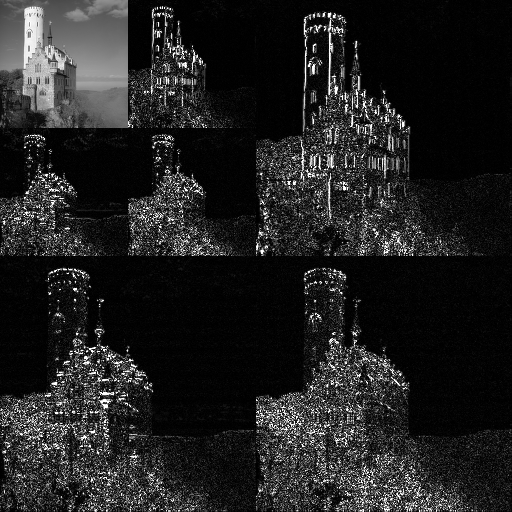
\includegraphics[width=.7\textwidth]{doc/thesis/0_figures/jp2_jpeg/Jpeg2000_2-level_wavelet_transform-lichtenstein.png}
        \caption{Hierarchical structure of an image transformed with 2-level \gls{dwt} \cite{Commons20192-levelTransform-lichtenstein}.}
        \label{fig:jp2_hierarchy}
\end{figure}

A comparison of an image compressed with \gls{jpeg} and with \gls{jp2} with roughly similar compression ratio is presented in Figure~\ref{fig:jpg_jp2_comparison}. Artefacts are created around the contours in the \gls{jpeg} image in contrast to the \gls{jp2} image, despite the higher compression ratio of the \gls{jp2} image.
\begin{figure}[htb]
    \centering
    \begin{subfigure}[b]{0.7\textwidth}
        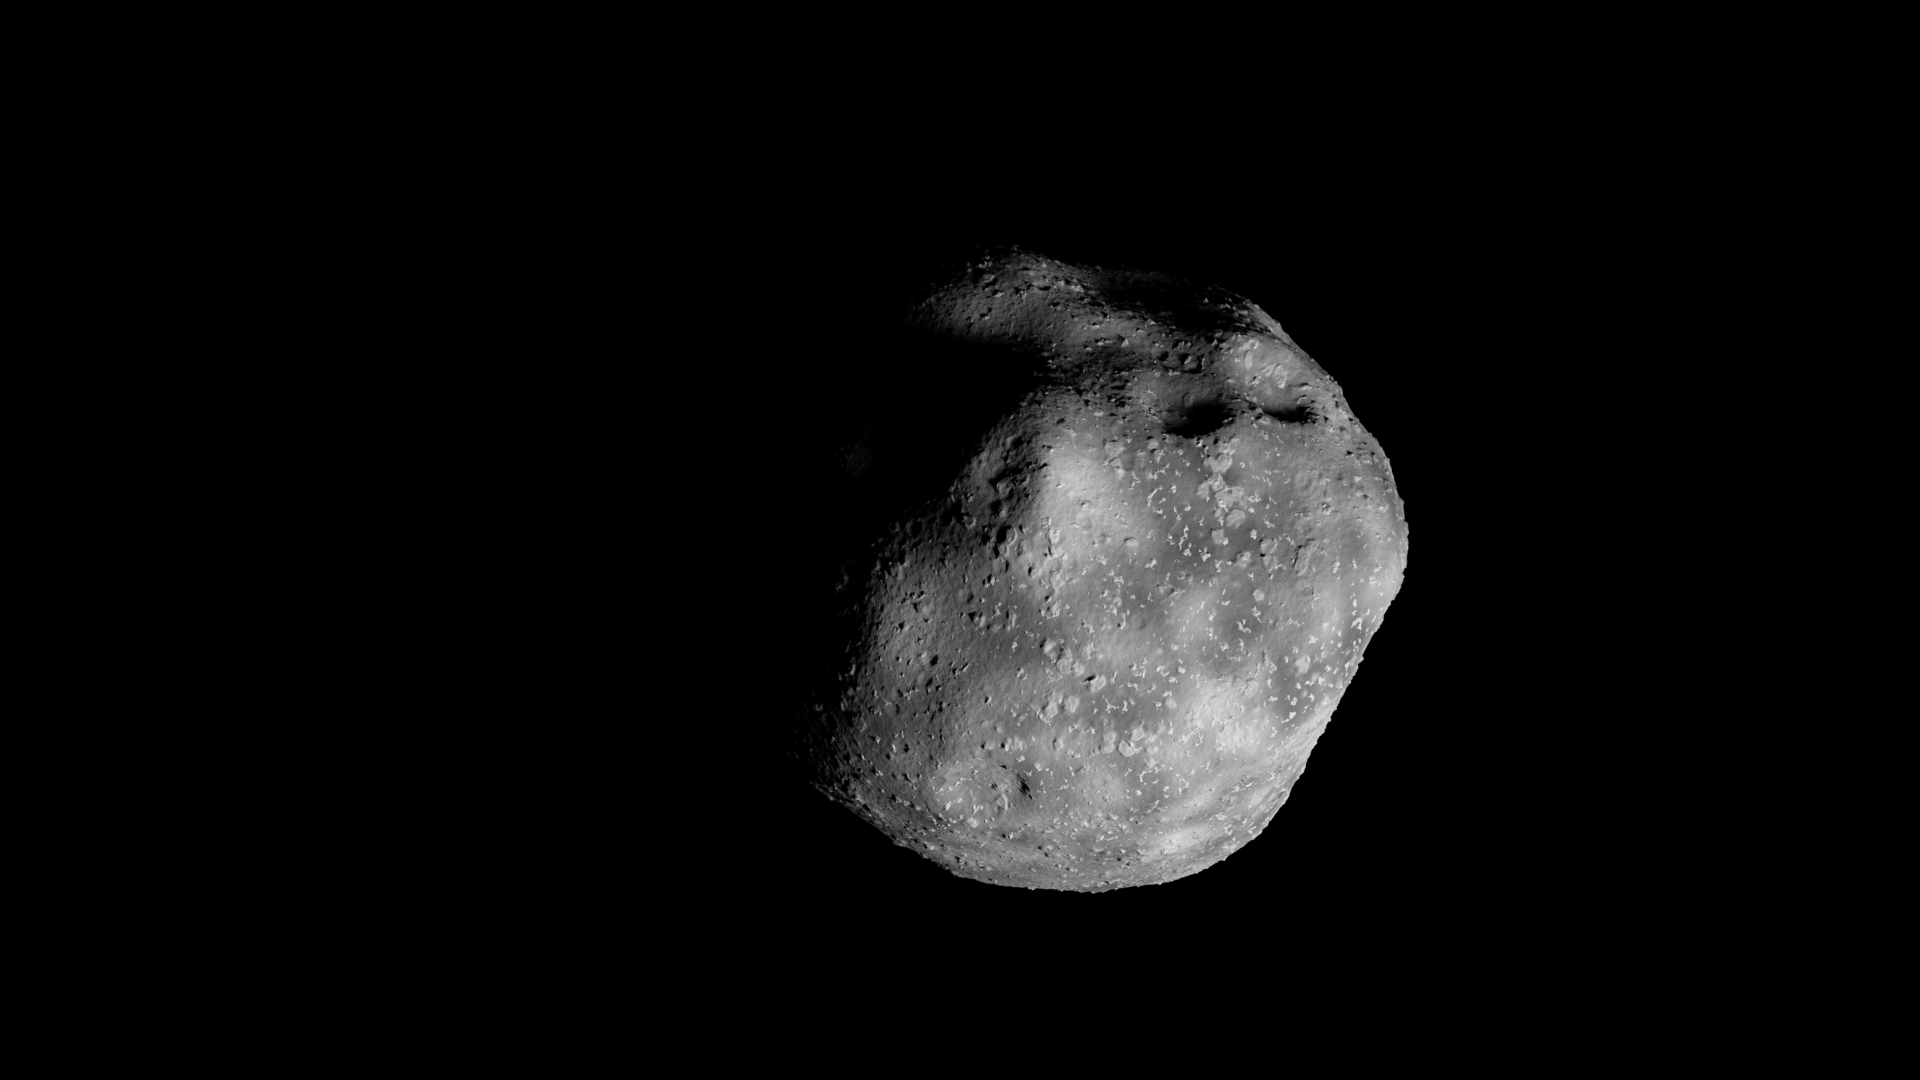
\includegraphics[width=\textwidth]{doc/thesis/0_figures/jp2_jpeg/orig.png}
        \caption{Original image without compression.}
        \label{fig:jpg_jp2_oirg}
    \end{subfigure}
    \\
    \begin{subfigure}[b]{0.48\textwidth}
        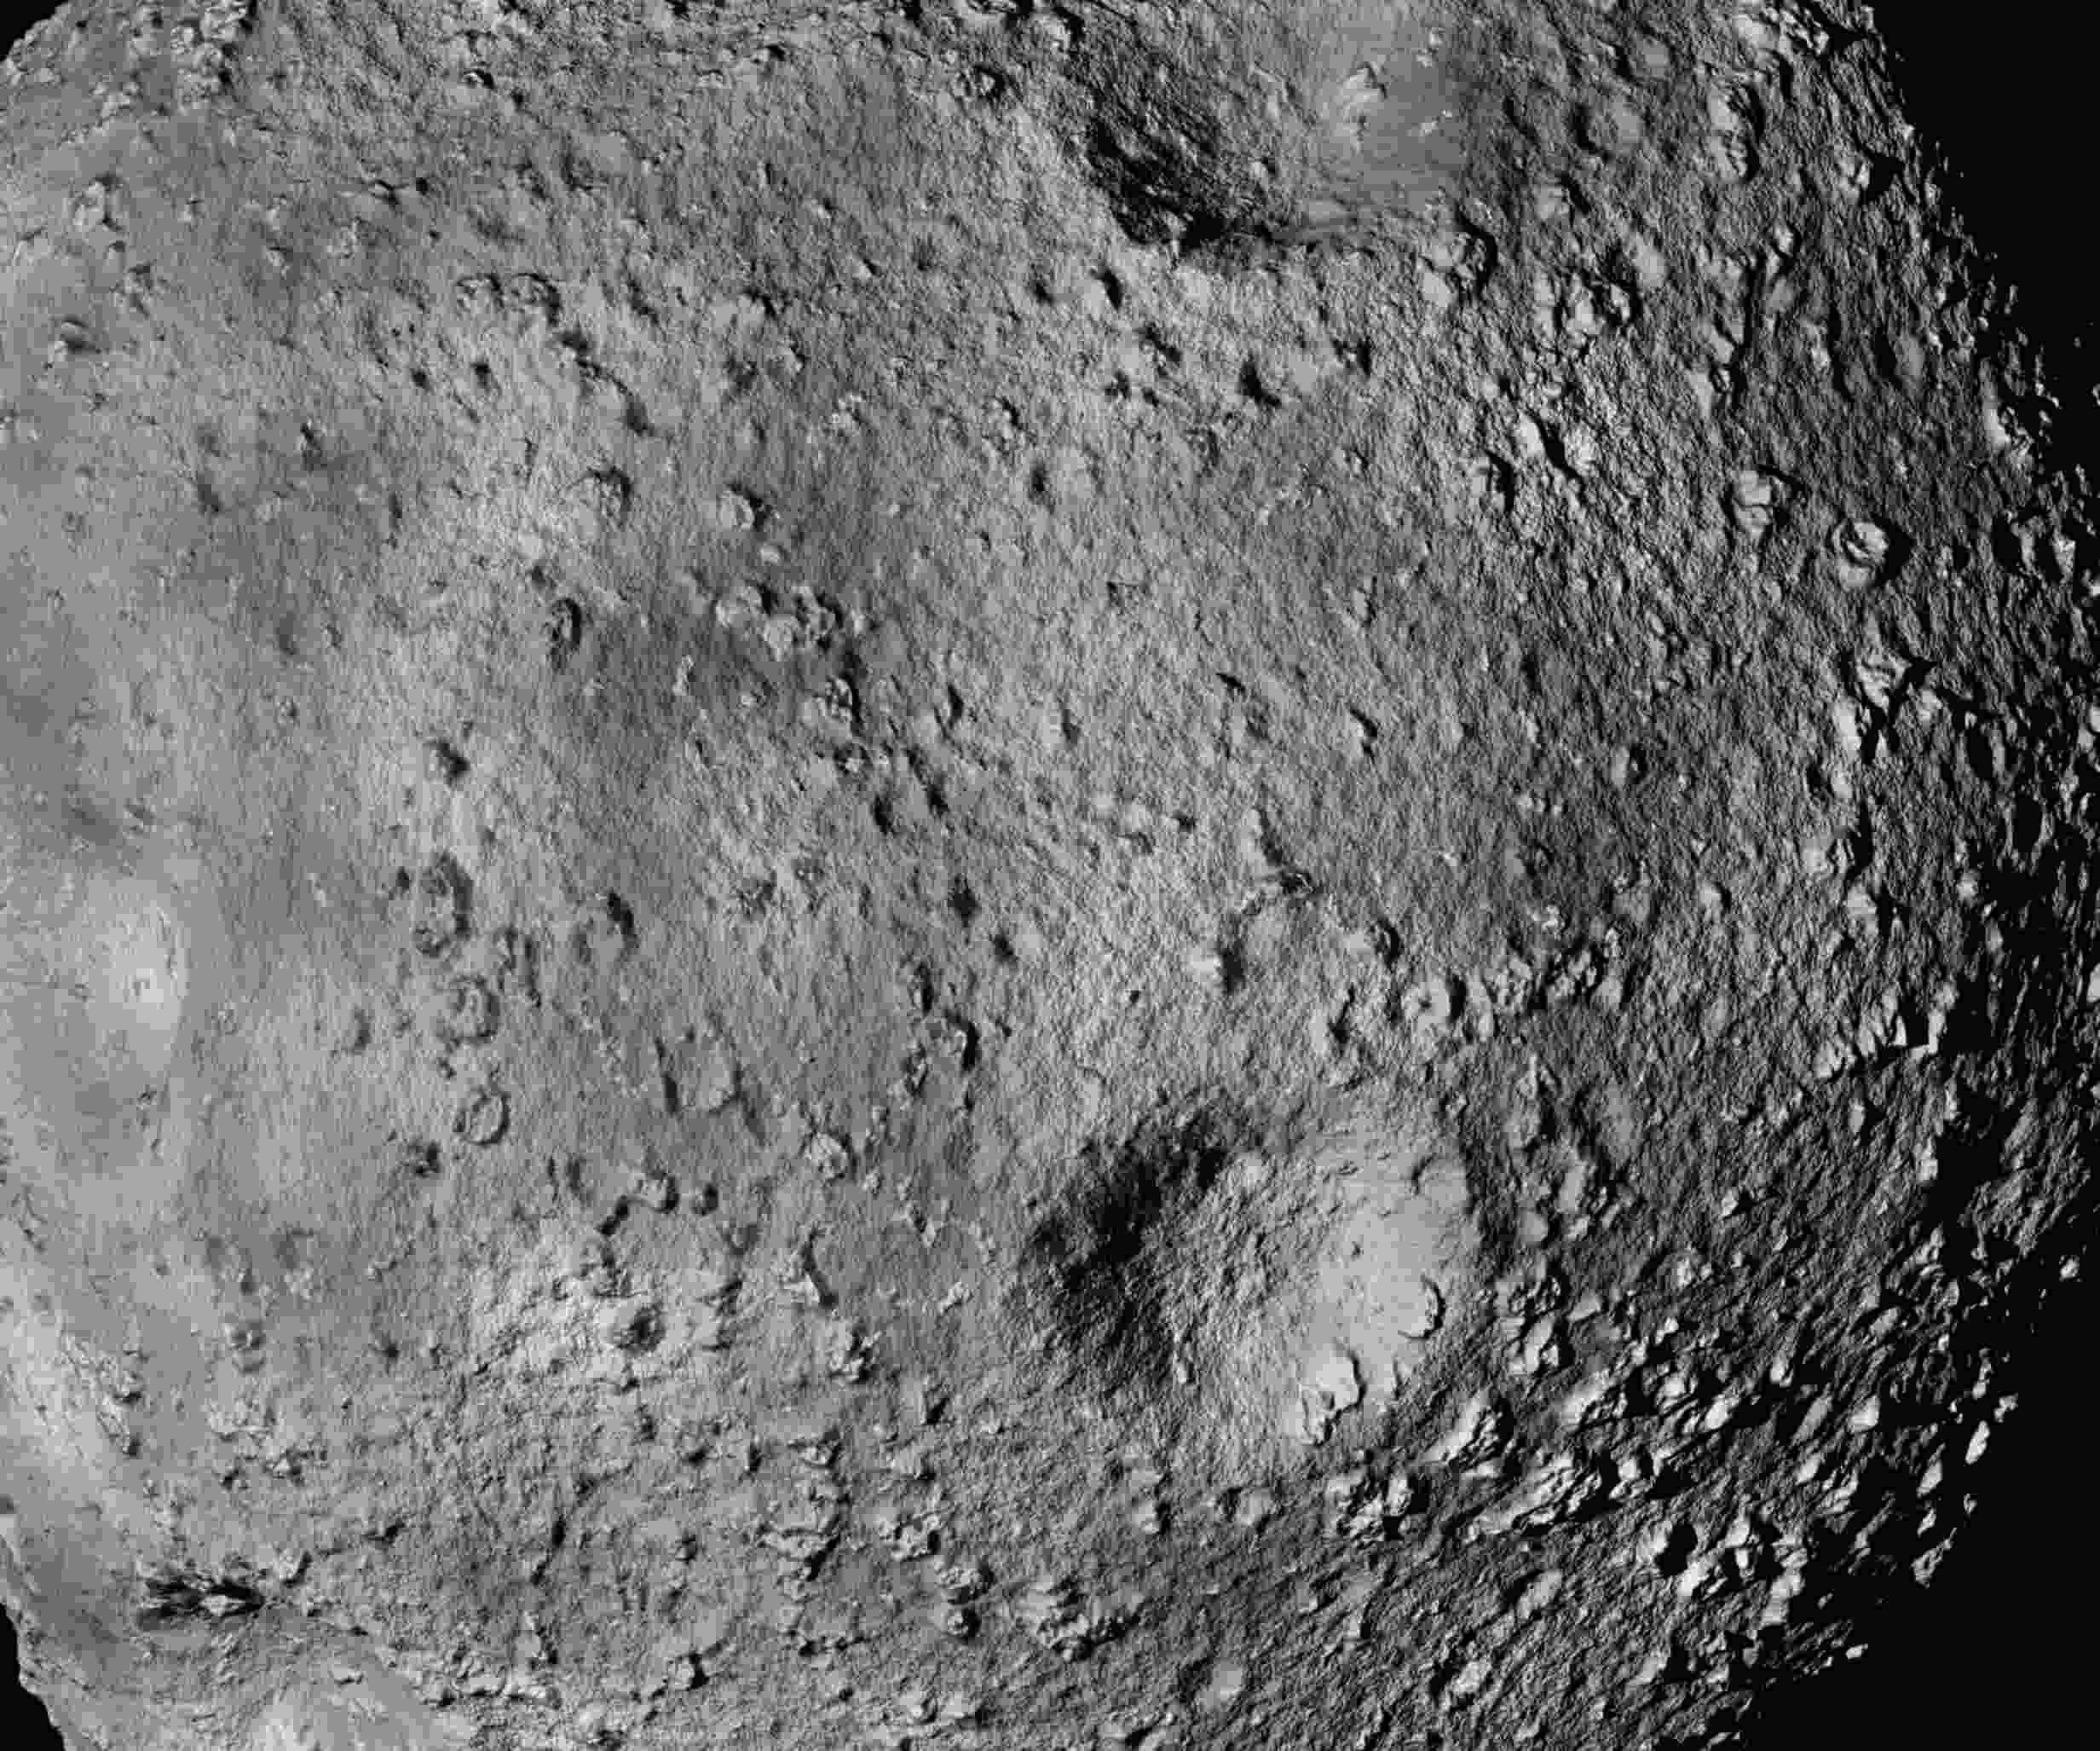
\includegraphics[width=\textwidth]{doc/thesis/0_figures/jp2_jpeg/proc_5.jpg}
        \caption{}
        \label{fig:jpg_jp2_jpeg}
    \end{subfigure}
    \begin{subfigure}[b]{0.48\textwidth}
        \includegraphics[width=\textwidth]{doc/thesis/0_figures/jp2_jpeg/proc_11.png}
        \caption{}
        \label{fig:jpg_jp2_jp2}
    \end{subfigure}
    \caption{Comparison of images compressed with \gls{jpeg} and \gls{jp2}. Despite a higher compression ratio, the \gls{jp2} image produces a better result for a \gls{sssb} image. (a)~Raw image without compression. (b)~Image compressed with \gls{dct} using the \gls{jpeg} format with a compression ratio of 61.2:1. (c)~Image compressed with \gls{dwt} using the \gls{jp2} format with a compression ratio of 64.3:1.}
    \label{fig:jpg_jp2_comparison}
\end{figure}

\subsubsection{Gaussian Filtering} \label{sec:t_gauss}
Gaussian filtering convolves an image with a \gls{2d} Gaussian distribution function. The effect of Gaussian filtering is blurring which removes noise and details. The \gls{2d} Gaussian function \gls{G}$(x,y)$ with a mean of zero is defined as
\begin{align}
    G(x,y) = \frac{1}{2\pi \sigma^{2}}e^{-\frac{x^2+y^2}{2\sigma^2}}, \label{eq:gauss_2d}
\end{align}
where \gls{sigma} is the standard deviation of the Gaussian distribution, and $x$ and $y$ are coordinates. The Gaussian distribution theoretically extends to infinity. Practical implementations cut the Gaussian distribution at a certain distance from the centre. The kernel size determines the range over which the filter is applied. Since \SI{99}{\percent} of the distribution falls within three standard deviations, the kernel size is related to the standard deviation of the Gaussian distribution. Furthermore, the Gaussian distribution is discretised in a digital system. The \gls{2d} Gaussian filter is rotationally symmetric and larger standard deviation creates a stronger blurring effect due to a wider peak.

\subsubsection{Down-sampling with Local Means} \label{sec:t_downsample}
Down-sampling is the process of reducing the number of pixels in an image. Down-sampling with local means refers to replacing a set of pixels with a single pixel having the average value of the pixel set. If an image is reduced by a factor of two, the values of four pixels are averaged to obtain a single output pixel. In the example in Figure~\ref{fig:downsample_example}, a $4\times4$ matrix is down-sampled by a factor of two resulting in a $2\times2$ matrix.
\begin{figure}[htb]
    \begin{align*}
        \begin{bmatrix}
            1  & 2  & 3  & 4\\
            5  & 6  & 7  & 8\\
            9  & 10 & 11 & 12\\
            13 & 14 & 15 & 16\\
        \end{bmatrix} 
        \rightarrow 
        \begin{bmatrix}
            3.5  & 5.5\\
            11.5 & 13.5\\ 
        \end{bmatrix}
    \end{align*}
    \caption{A $4\times4$ matrix down-sampled with local means by a factor of two resulting in a $2\times2$ matrix}
    \label{fig:downsample_example}
\end{figure}
